%
% introduction.tex
%
% Copyright (C) 2023 by Gabriel Mariano Marcelino.
%
% Towards the Conception of GNSS Networks Based on Small Satellites
%
% This work is licensed under the Creative Commons Attribution-ShareAlike 4.0
% International License. To view a copy of this license,
% visit http://creativecommons.org/licenses/by-sa/4.0/.
%

%
% \brief Introduction slides.
%
% \author Gabriel Mariano Marcelino <gabriel.mm8@gmail.com>
%
% \version 1.0.0
%
% \date 2023/09/07
%

\begin{frame}{Introduction}

    \begin{itemize}
        \item This work proposes the study, feasibility verification, and implementation of a network of a Global Navigation Satellite System (GNSS) based on small satellites, especially nanosatellites, or specifically CubeSats
    \end{itemize}

\end{frame}

\begin{frame}{Nanosatellite Launches}

    \begin{figure}[!ht]
        \begin{center}
            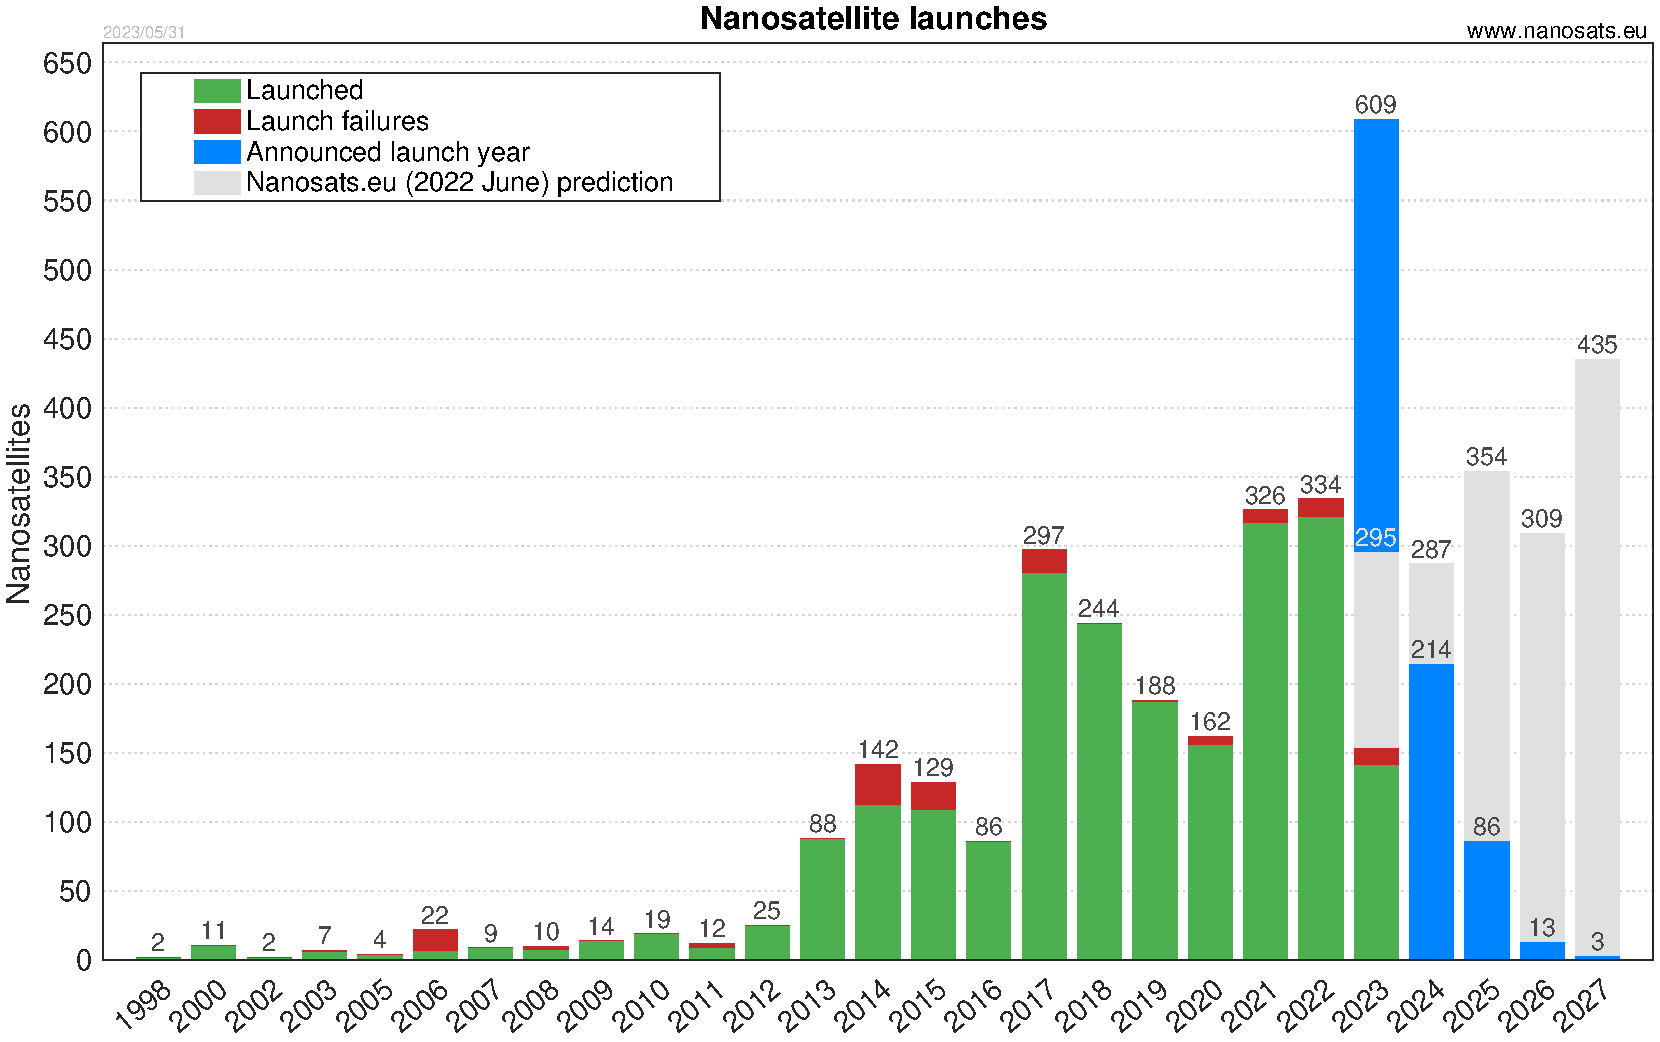
\includegraphics[width=0.9\columnwidth]{figures/Nanosats_years_2023-05-31}
        \end{center}
    \end{figure}

\end{frame}

\begin{frame}{Nanosatellite Constellations}

    \begin{figure}[!ht]
        \begin{center}
            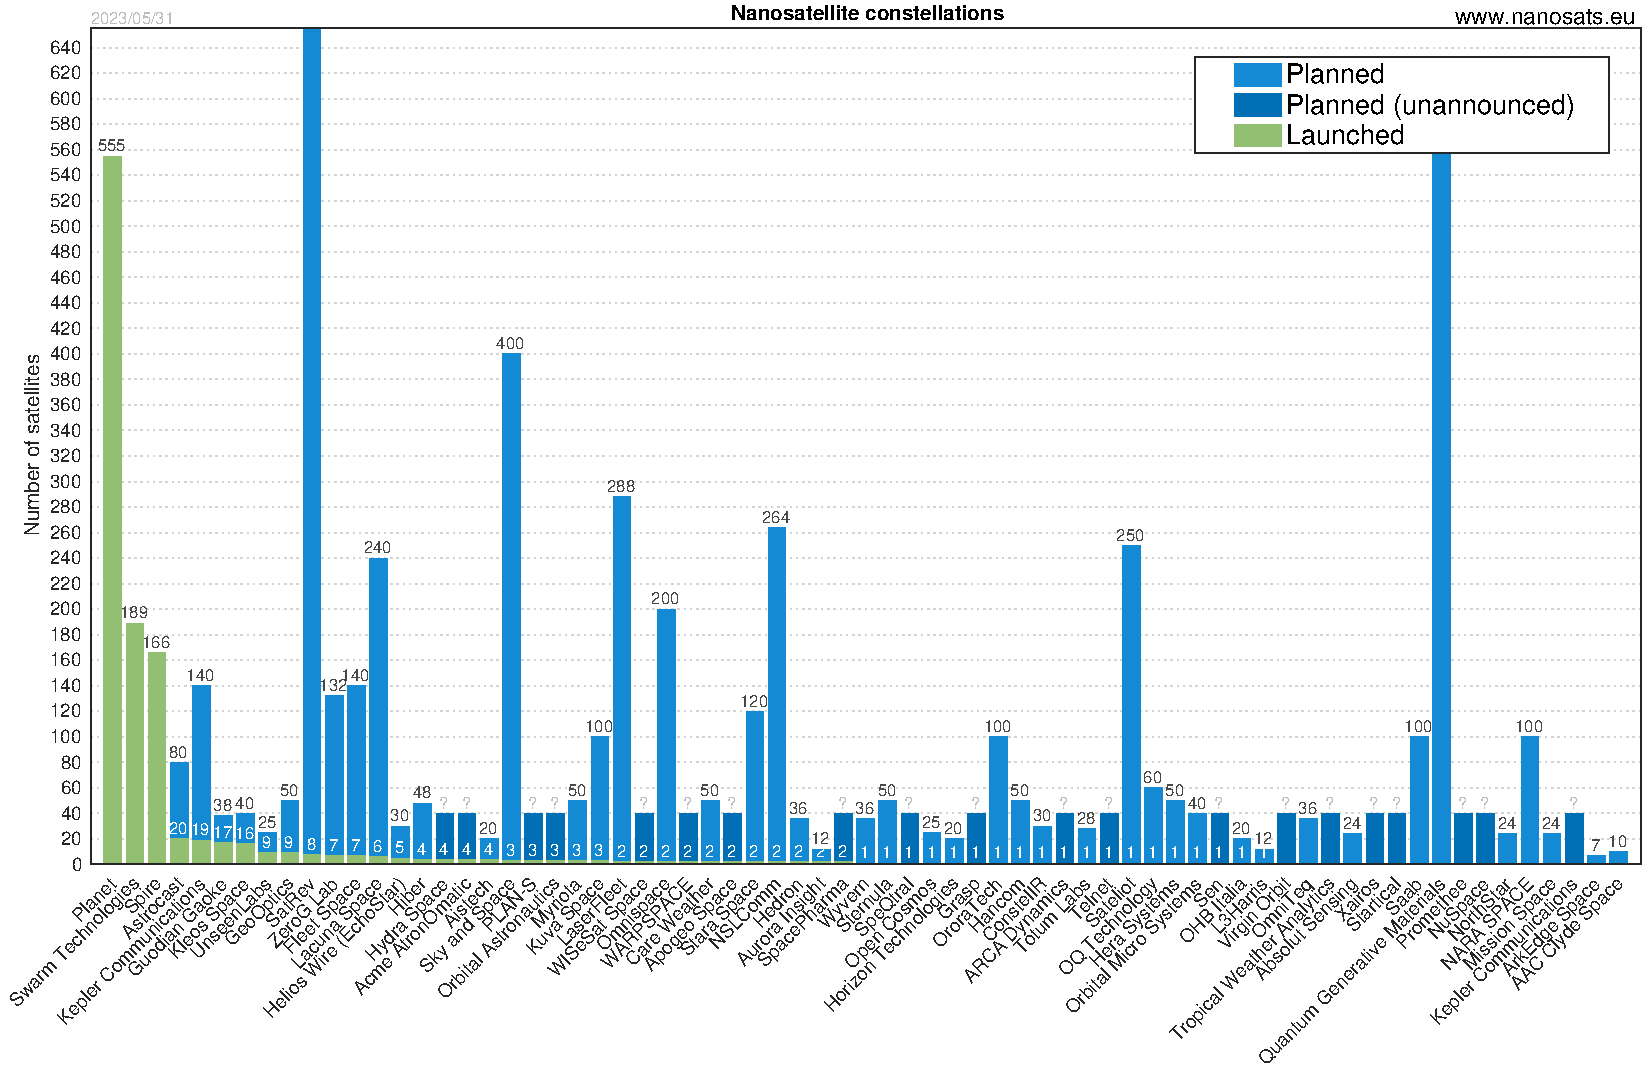
\includegraphics[width=0.9\columnwidth]{figures/Nanosats_constellations_2023-05-31}
        \end{center}
    \end{figure}

\end{frame}

\begin{frame}{Objectives}

    \begin{itemize}
        \item The main objective of this work is to evaluate the possibility and feasibility of deploying a geolocation system based on small satellites, mainly operating in the form of a low Earth orbit constellation
        \vspace{0.3cm}
        \item Another objective is to develop a payload for generating and transmitting GNSS signals, to be used on a small satellite in a mission designed specifically to test and verify the performance of the proposed system
    \end{itemize}

\end{frame}

\begin{frame}{Original Contribution}

    \begin{itemize}
        \item This work's main contribution is to evaluate the feasibility of implementing a geolocation system based on small satellites, exploring possible technologies that can be used to simplify and/or miniaturize the components involved in the space segment of such a system, a study of possible orbits and constellation sizes, and the necessary requirements for the system's satellites
    \end{itemize}

\end{frame}
